\chapter{Introdução}
\label{sec:introducao}

    \section{Contextualização}
	
	O desenvolvimento de software configura-se como uma atividade essencial no cenário atual, no qual empresas procuram se desenvolver digitalmente para manter sua competitividade no mercado \cite[]{cardoso2019and}. Nesse contexto, boas práticas tornam-se fundamentais para manter um projeto de qualidade, o que facilita sua escalabilidade e manutenção. 

    As boas práticas de desenvolvimento de software consistem em técnicas utilizadas antes e durante  a fase de desenvolvimento, visando garantir a qualidade, escalabilidade, manutenibilidade e segurança \cite[]{braga2007visao}. Alguns padrões utilizados na indústria de sistemas da informação é o versionamento de código com git, testes automatizados, criação de códigos genéricos para reutilizar, documentação clara, padrões de design, revisão de código, criação de diagramas da UML e planejamento de arquitetura bem detalhada. Apesar da existência dessas boas práticas, nem todo software acaba utilizando, como é o caso de projetos \textit{Go Horse} \cite[]{sturmaplicaccao}.

    O termo \textit{Go Horse} surgiu de maneira informal e humoristica no meio do desenvolvimento de software. Essa expressão, principalmente no Brasil, descreve projetos que foram conduzidos de forma improvisada, sem um planejamento prévio adequado, testes e documentações. Essa prática prioriza entregas rápidas, entretanto com pouca qualidade, resultando assim em falhas no sistema, difícil manutenção e elevados riscos para falhas de segurança, indo contra os padrões de metodologias ágeis \cite[]{perry2016funccao}. 

    Este trabalho tem como objetivo de estudo o software livre Web Gerenciador para Instituicões Assistenciais (WeGIA), que possui características típicas de um projeto \textit{Go Horse} e servirá de base de estudo e aplicação de boas práticas de desenvolvimento.
    
    O WeGIA foi desenvolvido pelos alunos do CEFET-RJ - campus Nova Friburgo. Sua criação surgiu pela falta de softwares \textit{Open Sources}, cujo seu objetivo central é melhorar a gestão, controle e transparência das entidades publicas. Sua versão atual possui seis módulos, dentre eles temos contribuição e sócios, material e patrimônio, memorando, pessoas, pet e saúde. \cite[]{latinoware2024wegia}
    
    \section{Problemas investigados}

    Projetos conduzidos sob a abordagem \textit{Go Horse} tendem a garantir sistemas que envelhecem rapidamente, tornando-se mais difícil de manter sua atualização e manutenção gradual. Esse fenômeno acaba gerando diversas soluções improvisadas durante o desenvolvimento. Aliada à falta de documentação, esses sistemas acabam se tornando rígidos, gerando um grau de complexidade elevado para a entrada de novos desenvolvedores na equipe e aumentando o risco de falhas a cada modificação realizada.
    
    Embora não seja um conceito formal na literatura acadêmica,  \textit{Go Horse} se relaciona com problemas amplamente discutidos nos dias atuais, como \textbf{dívida técnica}, \textbf{antipadrões de software}, \textbf{código legado} e \textbf{ad hoc}. Compreender o impacto no desenvolvimento de software evidencia a necessidade de aplicar boas práticas de desenvolvimento, garantindo que um projeto improvisado se transforme em um sistema sustentável e de fácil manutenção.

    O Wegia apresenta diversas características de um projeto com dívidas técnicas adquiridas no decorrer do tempo, tais como a falta de testes automatizados, tabelas sem normalização, código sem padrões estabelecidos, baixa segurança, documentação incompleta e uma arquitetura rígida. Essas características acabam impactando em retrabalho, demostivação da equipe e insatisfação de pessoas envolvidas.\cite[]{borges2022investigaccao}
    
    Por estar no mercado de código aberto, considera-se que novos usuario irão se utilizar e dar melhorias no projeto. Com isso, torna-se primordial a existencia de uma documentação clara e padrões de códigos pré estabelicidos, permitindo que o conhecimento sobre o software seja passada de forma fácil e prática entre membros da comunidade que se interessem pelo projeto.\cite[]{souza2010contribuiccao}

    Diante esse cenário e os problemas investigados, surge a questão de pesquisa desse trabalho: \textbf{Quais técnicas e boas práticas de desenvolvimento de software podem ser empregadas na refatoração de sistemas legados para garantir segurança, escalabilidade e facilidade de manutenção?}
        
    \section{Objetivos}
    \label{subsec:objetivos}

    Diante dos problemas associados ao desenvolvimento \textit{Go Horse}, a reestruturação de um software com tecnologias legadas e práticas inadequadas surge como uma solução estratégica. O objetivo geral é modernizar o sistema, aplicando boas práticas de programação, prevenindo o seu envelhecimento. Esse objetivo principal pode ser decomposto em objetivos especificos, como:

    \begin{itemize}
        \item Analisar o projeto atual do Wegia, identificando suas falhas, dívidas técnicas, código legado e vulnerabilidades de segurança;
        \item Reestruturar a aplicação, realizando a migração de uma aplicação em PHP puro para os frameworks Laravel no \textit{backend} e Nuxt no \textit{Frontend}, visando segurança e maior organização da estrutura do projeto;
        \item Implementar padrões e boas praticas de desenvolvimento, garantindo um projeto escalável e estavel;
        \item Propor uma arquitetura de software que promova modularidade, segurança e evolução contínua;
        \item Criar um script automático para facilitar a subida em servidores para fácil implementação;
        \item Elaborar um \textit{README} detalhado como forma de documentação técnica do projeto, tornando mais fácil e acessível para outros programadores darem início ao desenvolvimento;
        \item Utilizar ferramentas como o docker para facilitar o uso em qualquer sistema operacional;
        \item Realizar normalização das tabelas, quando necessário, migrando os dados do banco antigo para o novo;
        \item Validar o funcionamento da aplicação após sua migração tecnológica.
    \end{itemize}


    \section{Metodologia}

    Este trabalho se inspirou no modelo \textit{Design Science Research} \cite[]{pimentel2020dsr}, sendo adaptado conforme as necessidades específicas do projeto conforme ilustrado na Figura~\ref{fig:metodologia_utilizada}.:

    \begin{figure}[H]
        \centering
        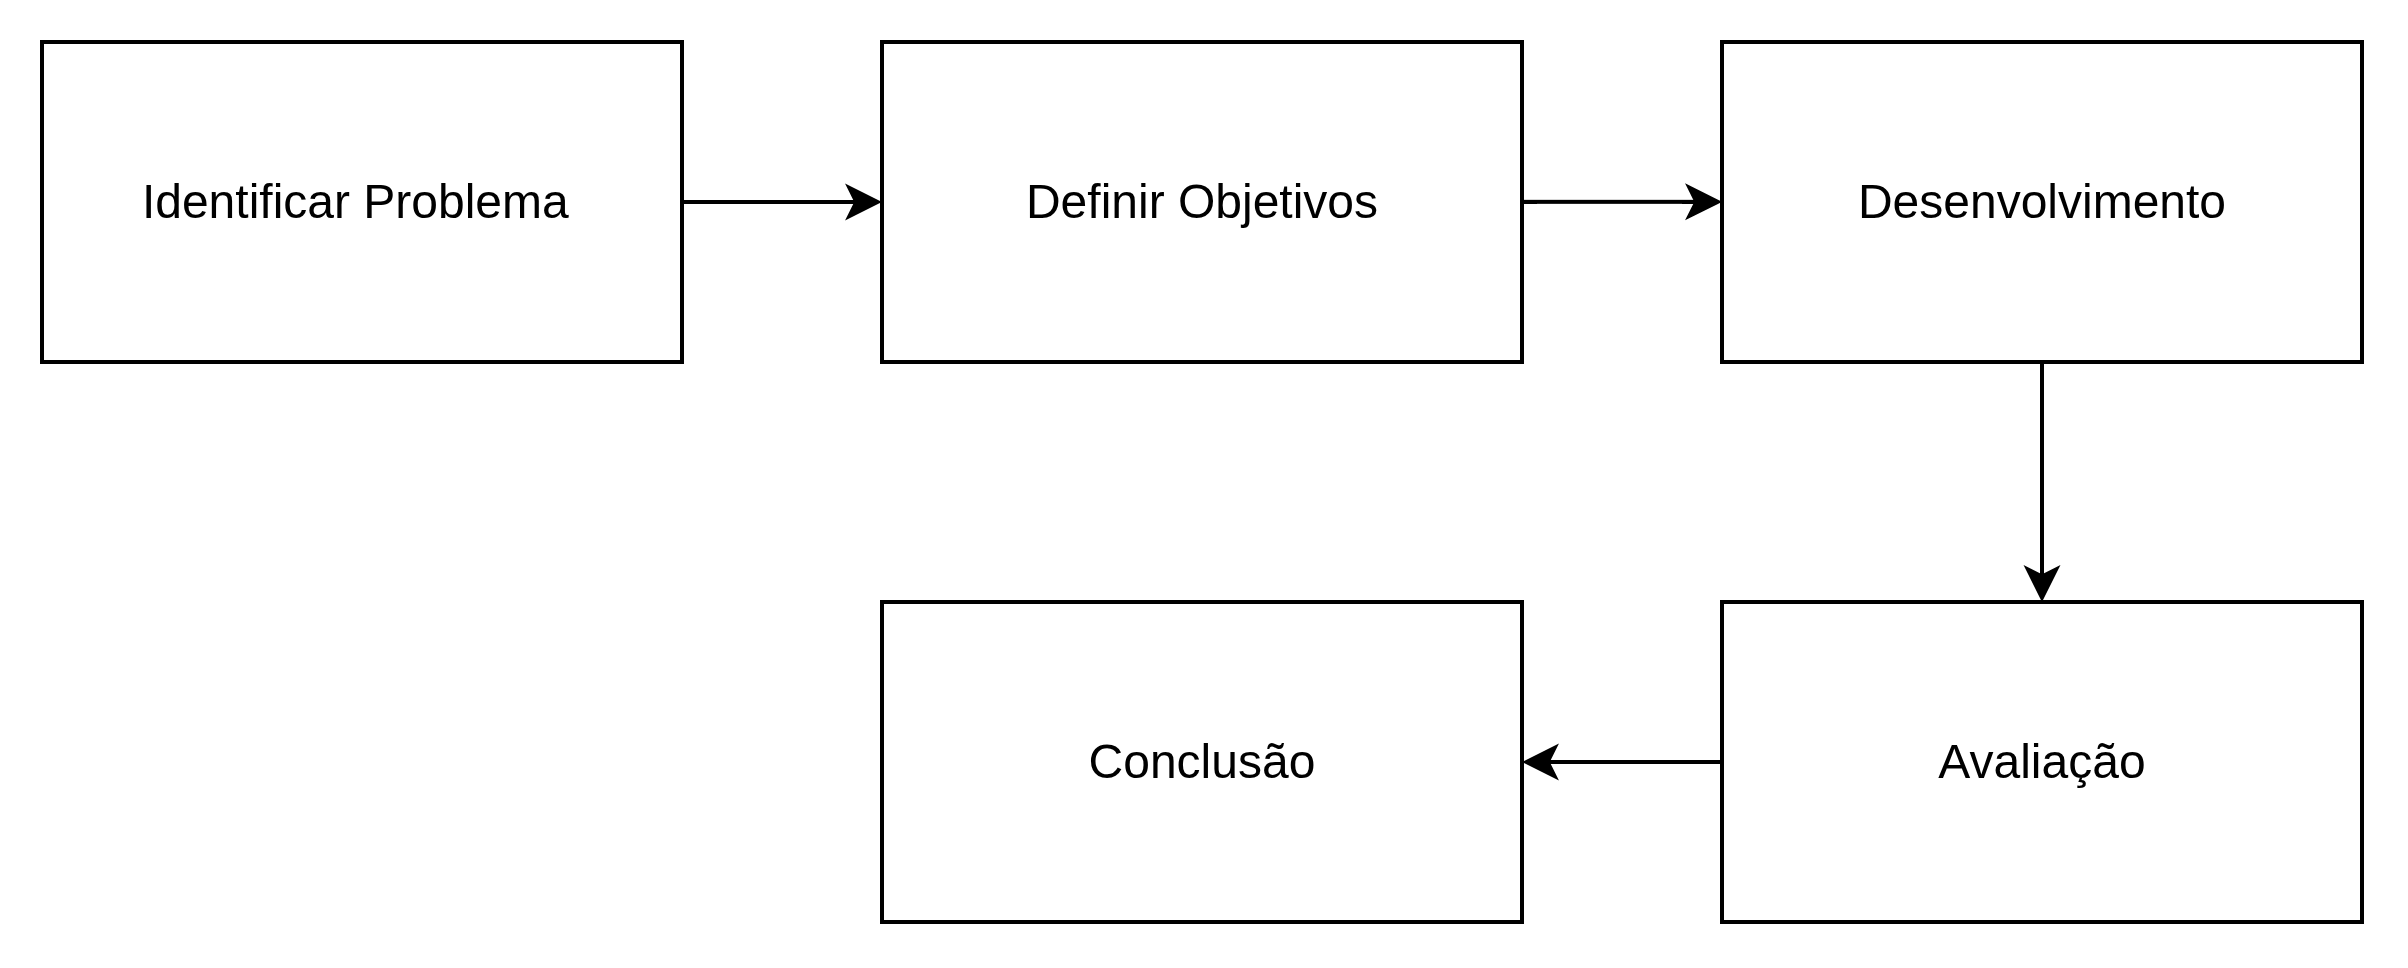
\includegraphics[width=1\linewidth]{imagens/Metodologia_utilizada.png}
        \caption{Fluxo metodológico utilizado e adaptado \citep{pimentel2020dsr} .}
        \label{fig:metodologia_utilizada}
    \end{figure}

     \begin{itemize}
        \item \textbf{Identificar Problema}:   
            Nesta Etapa, realizou-se uma analisada no atual código fonte do projeto do WeGIA e no seu banco de dados para buscar informações do que poderia ser melhorado. Além disso, teve um estudo conforme o artigo \cite[]{latinoware2024wegia} onde ocorreu uma pesquisa de campo para uma análise mais aprofundada das necessidades dos usuários no sistema.
        \item \textbf{Definir Objetivos}: 
            Esta etapa segue os objetivos citados dentro da introdução na subseção \ref{subsec:objetivos}, os quais orientaram a reconstrução do sistema na etapa de desenvolvimento. Para que fosse possível alcançar esse objetivo, foram utilizadas as tecnologias Laravel no backend e Nuxt.js no frontend, adotando padrões de arquitetura REST.
        \item \textbf{Desenvolvimento}: 
            Nessa etapa, foi realizada a migração tecnológica visando buscar um sistema com uma arquitetura modular, escalável, seguro e moderno.
        \item \textbf{Avaliação}: 
            O sistema após a reconstrução, foi submetido a diversos testes, como de carga e manuais, garantindo que todas suas funcionalidades estejam de acordo com o planejado.
        \item \textbf{Conclusão}:
            Os resultados obtidos na etapa de avaliação foi utilizada para revisar a solução proposta e identificar oportunidades de melhorias em cima dela.
    \end{itemize}

    \section{Organização do texto}
    
    Este projeto de conclusão de curso está dividio em cinco capítulos. O atual introduziu e contextualizou sobre o assunto abordado, evidenciando os problemas investigados e a questão de pesquisa

    O capítulo 2 aborda a  fundamentação teorica sobre o tema, servindo como  base para entendimentos dos demais capítulos.

    O Capítulo 3 apresenta os trabalhos relacionados, discutindo estudos anteriores sobre o tema de reestrutração de software.

    O Capítulo 4 descreve a proposta de solução do trabalho, apresentando caraterísticas, diagramação, tecnicas utilizadas, testes realizados e avalições descrito em mais detalhes.

    O capítulo 5 conclui o trabalho, apresentando uma discussão final sobre o tema, bem como sugestões de trabalhos futuros e considerações finais.
